% ESQUELETO DA DEFESA — estrutura apenas, sem conteúdo.
% Gerado a partir de PLANO_FLUXO_DEFESA.md §3, §8, §11 (2026-08-21).
% Nada de texto de slide entra aqui antes de 22/08 (plano validado com o orientador — ver §9).
% O showcase original do template (todos os comandos de exemplo: blocos, tabelas, código,
% algoritmos, equações, citações) foi preservado em template_showcase.tex — consulte-o para
% a sintaxe de qualquer recurso usado abaixo.

\documentclass{beamer}
\usepackage[net,green]{nesped}
\usepackage[brazilian]{babel}

% As figuras entregues vivem na arvore da dissertacao. graphicspath evita caminho longo em
% cada \includegraphics e mantem o .tex legivel.
\graphicspath{{img/}{../figures/plates/}{../../src/figures/}{../../src/figures/mobiwac/}{../../src/figures/courb/}}
\usepackage{booktabs}

% Titulo e nome copiados da folha de rosto do volume entregue (src/banca.pdf, p. 1),
% verificados por extracao de texto em 2026-08-23. Nao reescrever de memoria.
\title[Check-in-Level Representation]{Multitask Learning for Point-of-Interest Classification and Prediction Tasks: The Role of the Check-in-Level Representation}
\subtitle{Defesa de Dissertação de Mestrado --- PPGCC/UFV}
\author{Vitor Hugo de Oliveira Silva}
\institute[UFV]{Universidade Federal de Viçosa\\\smallskip\footnotesize Orientador: Fabrício Aguiar Silva}
\date{28 de agosto de 2026}

\setlength{\columnsep}{6mm}

\begin{document}

\begin{frame}{The architecture: sharing by exchange}
    \framesubtitle{Two inputs, one model}
    \begin{columns}[T,onlytextwidth]
        \begin{column}{0.62\textwidth}\centering
            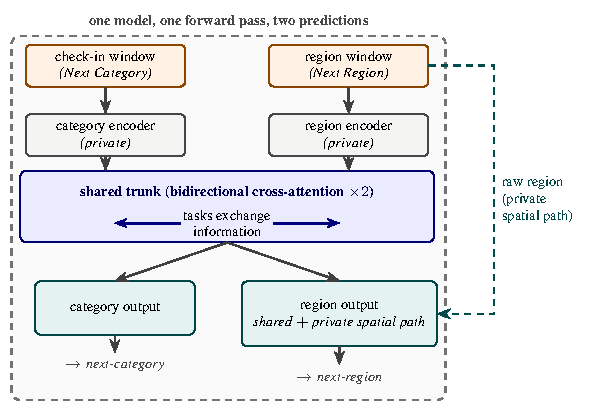
\includegraphics[width=\linewidth]{fig2_model_slides}
        \end{column}\hfill
        \begin{column}{0.345\textwidth}
            \vspace{2mm}
            {\footnotesize
            \textbf{Two inputs} $\cdot$ 9 visits $\times$ 64\,d each\\
            $\cdot$ Next Category --- per-visit vectors\\
            $\cdot$ Next Region --- same window
            \par\vspace{4mm}
            \textbf{Private encoders} --- no shared weights
            \par\vspace{4mm}
            \textbf{Shared trunk}\\
            2 cross-attention blocks\\
            4 heads $\cdot$ width 256
            \par\vspace{5mm}
            \alert{\textbf{One shared module, no shared hidden layers:}
            the two tasks \textbf{EXCHANGE}, they do not \textbf{MERGE.}}\par}
        \end{column}
    \end{columns}
\end{frame}

\end{document}
